\section{Solución Propuesta}

\subsection{Descripción General}
La solución desarrollada se organiza en un componente central, una aplicación móvil y nodos periféricos de balanzas y tracking. El componente central cuenta con un frontoffice web con una sección pública y áreas de acceso autenticado para empresas transportistas y funcionarios, y un backoffice para autoridades y administradores. Estas interfaces ofrecen funcionalidades de gestión de empresas, vehículos y viajes, fiscalización, consulta de reportes y administración de usuarios. La Figura \ref{fig:descripcion-general} presenta una vista general de la plataforma, sus usuarios y los sistemas externos con los que se integra. A continuación, se describen los principales aspectos de la solución.

\begin{figure}
\centering
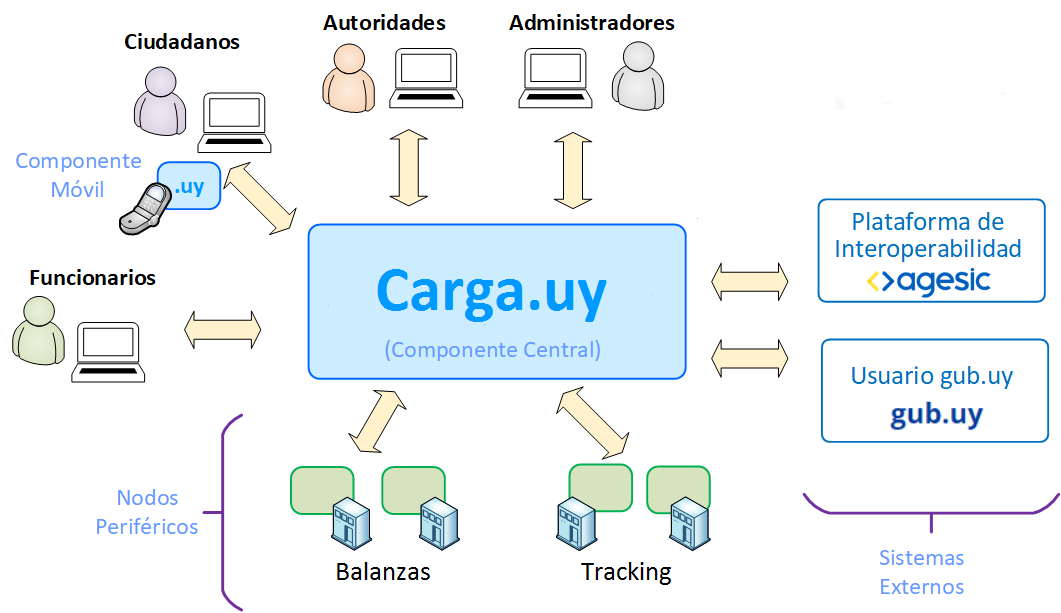
\includegraphics[width=\textwidth]{figuras/descripcion-general.png}
\caption{Descripción General de la Solución} \label{fig:descripcion-general}
\end{figure}


\subsection{Gestión de empresas, vehículos y viajes}
El frontoffice permite a los responsables gestionar la información de su empresa, sus vehículos y las guías de carga. A partir de una guía se asigna un viaje a un vehículo y un chofer de la empresa, comprobando la vigencia de sus habilitaciones y del vínculo del chofer. Los permisos ingresados por el responsable quedan pendientes de revisión por un funcionario, quien puede aprobarlos indicando su período de validez o rechazarlos dejando un motivo. El acceso a estas operaciones se controla en la capa de servicios según el rol del usuario y su relación con la empresa.

\subsection{Autenticación y acceso}
El frontoffice y la aplicación móvil utilizan Usuario gub.uy mediante OpenID Connect. El componente central recibe el código de autorización y lo intercambia con gub.uy para obtener la identidad del usuario. A partir de su cédula busca el registro correspondiente y, si es un ciudadano que ingresa por primera vez, lo crea. Los roles se obtienen de la información registrada en el componente central.

El central genera un JWT propio firmado, cuyos claims incluyen el identificador del usuario, la cédula, los roles, el correo cuando está disponible, el emisor, el tipo de token y las fechas de emisión y vencimiento. En el frontoffice se guarda en una cookie HttpOnly que acompaña las solicitudes. El central verifica la firma, la vigencia, el emisor y el tipo del token para identificar al usuario y sus roles.

La aplicación móvil realiza el ingreso desde el navegador, pero no comparte automáticamente sus cookies. Para obtener su token utiliza un intercambio con PKCE: genera y guarda un valor aleatorio, llamado code\_verifier, calcula su SHA-256 para obtener el code\_challenge y lo envía al endpoint de autenticación del central mediante el navegador. Tras completar el ingreso con gub.uy, el central devuelve a la aplicación un código temporal asociado al challenge. La aplicación envía ese código junto con el verifier al central, que verifica la validez del código y calcula nuevamente el SHA-256 del verifier para comprobar que coincida con el challenge antes de entregar el JWT.

Para las autoridades y los administradores, el backoffice utiliza un directorio LDAP, cuyos grupos determinan los roles de acceso. La administración de las cuentas del backoffice se realiza desde la propia aplicación.

\subsection{Aplicación móvil}
La aplicación móvil está destinada a los choferes. Tras el ingreso, descarga los viajes asignados y en curso del chofer junto con su Guía y los guarda en una base de datos local, de modo que puede consultarlos y operar sin conectividad. Desde el detalle de un viaje, el chofer registra el inicio y el fin, las cargas y descargas parciales con sus kilos y los incidentes con una descripción. La aplicación solo ofrece las acciones válidas para el estado del viaje y valida los datos con las mismas reglas que el componente central. Para que pueda seguir trabajando sin conexión, la sesión se mantiene con un token de renovación ligado a una clave del dispositivo guardada en el Android Keystore, por lo que una copia de ese token no sirve en otro equipo.

Cada evento se guarda primero en el dispositivo, con un identificador UUID generado localmente y la hora en que ocurrió, y luego se envía al central en segundo plano. El envío es una tarea que espera a que haya conexión, se ejecuta aunque la aplicación esté cerrada y, si falla, se reintenta con esperas crecientes. El central procesa cada evento en una transacción propia, de modo que uno inválido no afecta a los demás, y responde con un resultado por evento: aplicado, duplicado, en conflicto o rechazado. Como el identificador lo genera el dispositivo, un evento reenviado tras perderse la respuesta se reconoce como duplicado y no se aplica dos veces. El estado del viaje lo decide el central: un evento sobre un viaje que ya no pertenece al chofer se registra como conflicto, y uno incompatible con el estado del viaje o fuera de su horario, como rechazado. En ambos casos el evento se conserva y el chofer ve el motivo en la aplicación. Los eventos se aplican según la hora en que ocurrieron y no la de llegada, por lo que un inicio registrado sin conectividad fija la hora de inicio real y permite asociar al viaje las posiciones de tracking recibidas antes.

\subsection{Integración con balanzas}
La integración con balanzas se realiza mediante nodos periféricos que simulan los sistemas de los operadores de peajes. Cada nodo mantiene la información de sus peajes, balanzas y pesajes, y permite consultar las lecturas de un vehículo para una fecha determinada. Para obtener los pesajes de un viaje, el componente central consulta en paralelo los nodos habilitados y selecciona las lecturas correspondientes al horario del viaje. Cada pesaje se identifica mediante el nodo, la balanza y el identificador del registro original, para evitar duplicados al repetir las consultas. Si falla la consulta a un nodo, el central devuelve los resultados obtenidos de los demás e identifica los nodos que no pudieron consultarse.

\subsection{Generación asíncrona de reportes}
La exportación de reportes se realiza en segundo plano, de modo que la autoridad pueda solicitar un informe y volver más adelante para descargarlo. Al solicitarlo, se guardan los filtros seleccionados, el formato y el usuario solicitante, y el informe queda en estado pendiente. La solicitud se envía a una cola para su procesamiento. Cuando finaliza la generación, el archivo queda disponible en CSV o PDF en la sección de exportaciones del usuario. Si la generación falla, se registra ese estado y la autoridad puede realizar una nueva solicitud. Cada autoridad puede consultar y descargar únicamente sus propias exportaciones.


\subsection{Ingesta de eventos de tracking}
Los nodos de tracking no invocan al componente central: publican las posiciones en una cola del broker de mensajería, por TLS y con un usuario propio por nodo que solo puede publicar en esa cola. Si el central no está disponible o recibe más posiciones de las que puede procesar, estas esperan en la cola, y ante una saturación el broker las guarda en disco en lugar de descartarlas.

En el central, un Message-Driven Bean consume las posiciones, descarta las de nodos no registrados o deshabilitados y almacena el resto en una base de datos documental. Un índice único por nodo e identificador de evento evita guardar dos veces una posición reenviada. Cada posición se asocia al viaje que el vehículo tenía en curso cuando se generó, no cuando llegó: así, una posición demorada por falta de cobertura queda en su viaje. Si el chofer inicia el viaje sin conectividad, las posiciones previas al aviso de inicio se reasocian al viaje cuando este llega. Esto evita detectar viajes sin Guía que no lo son. Confirmada la transacción, el central dispara en segundo plano la evaluación de las reglas de fiscalización.

Si el procesamiento falla, por ejemplo porque la base de datos no responde, el broker reentrega la posición con una espera creciente, de uno a sesenta segundos, durante unos catorce minutos; si todos los intentos fallan, la posición pasa a una cola de mensajes muertos, desde la que puede reprocesarse. Varias instancias del central pueden consumir la misma cola para escalar la ingesta.

\subsection{Fiscalización automática}
\textcolor{red}{[Completar: reglas evaluadas, disparo desde la ingesta y desde el fin del viaje, deduplicación de casos, reevaluación ante balanzas no disponibles y ciclo del caso.]}

\subsection{Gestión de nodos periféricos}
El administrador registra cada nodo periférico desde el backoffice con su identificador, tipo y punto de acceso; para los nodos de balanzas, también la clave con la que el central se autentica, que se guarda cifrada. Todo nodo nuevo queda deshabilitado hasta que el administrador lo habilita, y vuelve a deshabilitarse si cambia su punto de acceso, porque un nodo mal configurado no produce errores visibles: el central aceptaría posiciones de una fuente no verificada o consultaría una dirección incorrecta.

\subsection{Observabilidad}
La plataforma utiliza OpenTelemetry. WildFly instrumenta automáticamente los servicios REST y las llamadas a otros sistemas; donde el contexto no se propaga solo, se pasa en forma explícita: en las propiedades de cada mensaje JMS, en la evaluación de reglas en segundo plano y en las consultas en paralelo a los nodos de balanzas. La aplicación móvil también envía el contexto en cada solicitud. Así, el fin de un viaje registrado desde el celular puede seguirse en una sola traza que incluye la sincronización, la evaluación de las reglas y la consulta a cada nodo de balanzas. Los logs incluyen el identificador de la traza. La telemetría se envía por OTLP a una plataforma con Prometheus, Tempo, Loki y Grafana, donde un tablero reúne las métricas de la ingesta, la cola, los nodos, la API, las integraciones y los health checks.
